% IEEE AIPR 2025 Paper - Improved Mathematical Notation
% Clear definitions of 2D wavelets and spatial coordinates
%
\documentclass[runningheads]{llncs}
%
\usepackage[T1]{fontenc}
\usepackage{graphicx}
\usepackage{amsmath,amssymb}
\usepackage{booktabs}
\usepackage{hyperref}
\usepackage{fontawesome5}
\begin{document}
%
\title{Wavelet Scattering Features based Colon Cancer Histology Classification}
%
\author{Ritish Raghav Maram\inst{1,2} \and
Elliot Levy\inst{2} \and
Murray Loew\inst{1}}
%
\authorrunning{R. R. Maram et al.}
%
\institute{The George Washington University, Department of Biomedical Engineering,\\
Washington DC, United States\\
\email{rmaram33@gwu.edu, loew@gwu.edu}
\and
National Institutes of Health, Clinical Center, Bethesda MD, United States\\
\email{levyeb@cc.nih.gov}}
%
\maketitle
%
\begin{abstract}
Histological evaluation of tumors plays an important role in malignancy identification and, more recently, in stratification of treatment response and prognosis. Quantitative imaging methodology has been applied to cross-sectional imaging datasets with pathology correlation to model tumor composition and tissue classification. Several digital image analysis studies have demonstrated prognostic significance for tumor heterogeneity, proportional representation of complex stroma, and immune cell infiltration. Texture analysis has been used for classification of several tissue subtypes. We examine here the use of wavelet transformations of images, which can optimize spatial and frequency distributions for the characterized intratumoral tissues. We have developed and evaluated a model for colon intratumoral tissue classification using wavelet scattering features, achieving 85.10\% accuracy on test data with precision (85.19\%), recall (85.10\%), and F1-score (85.08\%) across eight tissue types.

\keywords{Wavelet Scattering \and Tumor heterogeneity \and Colon Cancer \and Quantitative Imaging}
\end{abstract}
%
%
\section{Introduction}

Colorectal cancer classification depends in part on the tissue type as identified in histology images. Extracting descriptors from those images is an essential step in the process of characterizing the tissue. Previous work in colorectal cancer tissue classification has used a variety of features derived principally from classical image analysis tools~\cite{mezheyeuski2016image,zhou2019immune,lubner2015ct,jin2022combinatory,alic2014quantification,kather2016multi}. In this work, we apply the wavelet scattering transform, a wavelet-based method for feature extraction. While the scattering transform has recently demonstrated success in retinal OCT analysis~\cite{baharlouei2023wavelet} and fundus imaging~\cite{agboola2023wavelet} for disease classification, this work represents its first application to histopathology tissue classification. The transform has a sound mathematical basis and shares structural similarities with convolutional neural networks (CNNs). Unlike CNNs, however, the transform requires no training, is computationally efficient, and yields features that are explainable. We show that the features it generates perform well in tissue classification.

The continuous wavelet transform is foundational to understanding the construction of scattering transform coefficients. In this study, we use the complex Morlet wavelet family to compute the wavelet transform. Morlet wavelets, also known as Gabor wavelets, are defined as the product of a Gaussian envelope and a complex exponential~\cite{mallat2008wavelet}:
\begin{equation}
\psi_{\lambda,\theta}(\mathbf{x}) = e^{i\boldsymbol{\zeta}_{\lambda,\theta} \cdot \mathbf{x}} e^{-\|\mathbf{x}\|^2/(2\sigma^2)} + \epsilon(\mathbf{x})
\end{equation}
where $\boldsymbol{\zeta}_{\lambda,\theta}$ is the center frequency vector determined by scale $\lambda$ and orientation $\theta$. The Gaussian term $e^{-\|\mathbf{x}\|^2/(2\sigma^2)}$ gives the wavelet its localized shape, while $e^{i\boldsymbol{\zeta}_{\lambda,\theta} \cdot \mathbf{x}}$ represents a complex exponential with central frequency $\boldsymbol{\zeta}_{\lambda,\theta}$. The correction term $\epsilon(\mathbf{x})$ ensures the wavelet has zero mean (admissibility condition), and the parameter $\sigma$ controls the trade-off between spatial and frequency localization. This construction enables Morlet wavelets to serve as bandpass filters localized in both space and frequency, as demonstrated in Figure~\ref{fig:morlet}.
\begin{figure}[ht]
\centering
\includegraphics[width=0.9\textwidth]{Images/1D_morlet.pdf}

\caption{Morlet wavelets at two distinct scales, with their corresponding frequency spectra. Larger scale corresponds to lower frequency (coarser features).}
\label{fig:morlet}
\end{figure}


\subsection{2D Wavelet Transform}

The 2D continuous wavelet transform decomposes an image by convolving it with a family of filters. The 2D convolution of image $f(\mathbf{x})$ with a filter $h$ at spatial location $\mathbf{x} = (x,y)$ is defined as:
\begin{equation}
(f \ast h)(\mathbf{x}) = \int_{\mathbb{R}^2} f(\mathbf{u}) h(\mathbf{x} - \mathbf{u}) \, d\mathbf{u}
\end{equation}
where $\mathbf{u} = (u,v) \in \mathbb{R}^2$ is the integration variable.

We employ two complementary filter types that partition the frequency domain. The scaling function $\phi$ is a lowpass filter that retains low-frequency content, capturing the coarse structure of the image. The Morlet wavelet $\psi_{\lambda,\theta}$ is a bandpass filter localized around a specific frequency band determined by scale $\lambda$, with orientation selectivity along angle $\theta$. By using wavelets at multiple scales and orientations, we cover the frequency domain with bandpass filters at different scales and directions, capturing complete frequency content when combined with the lowpass component.

The wavelet transform $\mathcal{W}f$ of image $f$ thus consists of one lowpass filter and a collection of bandpass filters:
\begin{equation}
\mathcal{W}f = \{f \ast \phi(\mathbf{x}), \, f \ast \psi_{\lambda,\theta}(\mathbf{x})\}_{\lambda,\theta}
\end{equation}
where the notation $\{\cdot\}_{\lambda,\theta}$ indicates the collection over all scales $\lambda$ and orientations $\theta$.
 Table~\ref{tab:notation} summarizes the notation used throughout this paper.


\begin{table}[h]
\centering
\renewcommand{\arraystretch}{1.3}
\setlength{\tabcolsep}{10pt}
\caption{Mathematical notation.}
\label{tab:notation}
\begin{tabular}{cl}
\toprule
\textbf{Notation} & \textbf{Definition} \\
\midrule
$f(\mathbf{x})$ & Image \\
$\psi_{\lambda,\theta}(\mathbf{x})$ & Morlet wavelet at scale $\lambda$ and rotation $\theta$ (bandpass filter) \\
$\phi(\mathbf{x})$ & Scaling function (lowpass filter) \\
$\mathcal{W}f$ & Wavelet transform of image $f$\\
$\lambda_1, \theta_1$ & Scale and rotation parameters for layer 1 \\
$\lambda_2, \theta_2$ & Scale and rotation parameters for layer 2 \\
$\ast$ & Convolution operator \\
$|\cdot|$ & Complex modulus \\
$S^m f$ & Scattering coefficients of order $m$ \\
\bottomrule
\end{tabular}
\end{table}


%
\section{Background}

This section provides an overview of how wavelet scattering features are constructed from the wavelet modulus transform.

\subsection{Zeroth-Order Scattering Coefficients}

The first step in computing a scattering transform is to obtain the zeroth-order scattering coefficient, denoted as $S^0f$, which is obtained by convolving the image with the lowpass filter:
\begin{equation}
S^0f = f \ast \phi(\mathbf{x})
\end{equation}

\subsection{First-Order Scattering Coefficients}

Lowpass filtering with $\phi$ removes high-frequency content. This information can be recovered by convolving the image with wavelets at different scales and orientations:
\begin{equation}
f \ast \psi_{\lambda_1,\theta_1}(\mathbf{x})
\end{equation}


These wavelet coefficients are complex-valued and sensitive to translations in the input~\cite{anden2019joint}. To achieve local translation invariance, we apply the complex modulus operation pointwise:
\begin{equation}
|f \ast \psi_{\lambda_1,\theta_1}(\mathbf{x})|
\end{equation}
followed by averaging via convolution with the scaling function:
\begin{equation}
S^1f(\lambda_1,\theta_1) = |f \ast \psi_{\lambda_1,\theta_1}(\mathbf{x})| \ast \phi(\mathbf{x})
\end{equation}
where each choice of $(\lambda_1, \theta_1)$ produces one first-order coefficient.

\subsection{Second-Order Scattering Coefficients}

The modulus operation $|f \ast \psi_{\lambda_1,\theta_1}(\mathbf{x})|$ creates new high-frequency content (due to the nonlinearity) that is lost when averaging with $\phi$. This information can be recovered in a second layer by convolving with wavelets from a second filter bank:
\begin{equation}
|f \ast \psi_{\lambda_1,\theta_1}(\mathbf{x})| \ast \psi_{\lambda_2,\theta_2}(\mathbf{x})
\end{equation}
Applying the modulus and averaging:
\begin{equation}
S^2f(\lambda_1,\theta_1,\lambda_2,\theta_2) = \big||f \ast \psi_{\lambda_1,\theta_1}(\mathbf{x})| \ast \psi_{\lambda_2,\theta_2}(\mathbf{x})\big| \ast \phi(\mathbf{x})
\end{equation}

Each combination of $(\lambda_1,\theta_1)$ and $(\lambda_2,\theta_2)$ produces one second-order coefficient. Each second-order coefficient corresponds to a specific path through the scattering network determined by $(\lambda_1,\theta_1)$ from the first layer and $(\lambda_2,\theta_2)$ from the second layer.

\subsection{General $m$-th Order Coefficients}

This construction generalizes to arbitrary depth. The $m$-th order scattering coefficients are:
\begin{equation}
S^mf = \Big\{\big| \cdots \big||f \ast \psi_{\lambda_1,\theta_1}(\mathbf{x})| \ast \psi_{\lambda_2,\theta_2}(\mathbf{x})\big| \cdots \ast \psi_{\lambda_m,\theta_m}(\mathbf{x})\big| \ast \phi(\mathbf{x})\Big\}_{\lambda_1,\theta_1,\ldots,\lambda_m,\theta_m}
\end{equation}
involving $m$ successive applications of wavelet convolution and modulus, followed by averaging.

The complete scattering transform $\mathcal{S}f$ is the collection of all scattering coefficients from all orders:
\begin{equation}
\mathcal{S}f = \{S^0f, S^1f, S^2f, \ldots, S^mf, \ldots\}
\end{equation}

The wavelet scattering transform was developed by Mallat~\cite{mallat2012group}, who proved its key properties: preservation of signal energy, contraction (L$^2$ stability), and stability to small deformations. Applications to audio~\cite{anden2011multiscale} and image classification~\cite{bruna2011classification} demonstrated the effectiveness of scattering features. More recently, scattering transforms have shown promise in medical imaging, achieving 94--97\% accuracy for retinal OCT disease classification~\cite{baharlouei2023wavelet} and 98\% accuracy for glaucoma detection from fundus images~\cite{agboola2023wavelet}, demonstrating the method's suitability for medical image classification.

%
\section{Data}

Histology images of colorectal cancer (CRC) were taken from a publicly available database~\cite{kather2016multi}. This dataset contains images and corresponding labels for eight tissue types that are commonly found in CRC histology whole-slide images. The images are hematoxylin and eosin (H\&E) stained and classified into tumor epithelium (Tumor), simple stroma (Stroma), complex stroma (Complex), immune cell conglomerates (Lympho), debris and mucus (Debris), mucosal glands (Mucosa), adipose tissue (Adipose), and background images (Empty).

For each tissue type, there are 625 non-overlapping tissue tiles of size $150 \times 150$ pixels, for a total of 5000 images. Sample images are shown in Figure~\ref{fig:tissues}.

\begin{figure}[h!]
\centering
\includegraphics[width=0.9\textwidth]{Images/Textures_Tissues.png}
\caption{Eight tissue types present in the CRC histology dataset. Images of a tissue type are realizations of a stochastic process associated with its texture.}
\label{fig:tissues}
\end{figure}

%
\section{Texture Classification}

A two-dimensional random field implies that each pixel location is associated with a random variable. The random field is stationary if all these random variables share the same statistical distribution, meaning their distribution is invariant across the entire field. Image textures can be modeled as realizations of 2D stationary processes. Here, we consider that each tissue type is associated with a 2D stationary process, and images of that tissue type are realizations of the process associated with that tissue type, as illustrated in Figure~\ref{fig:tissues}.

The work by Bruna and Mallat~\cite{bruna2013invariant} demonstrated that scattering coefficients can discriminate textures having identical second-order moments but different higher-order moments. Second-order scattering coefficients capture information up to 4th-order moments, enabling discrimination even when power spectra are identical, as shown in Figure~\ref{fig:spectrum}.

\begin{figure}[h!]
\centering
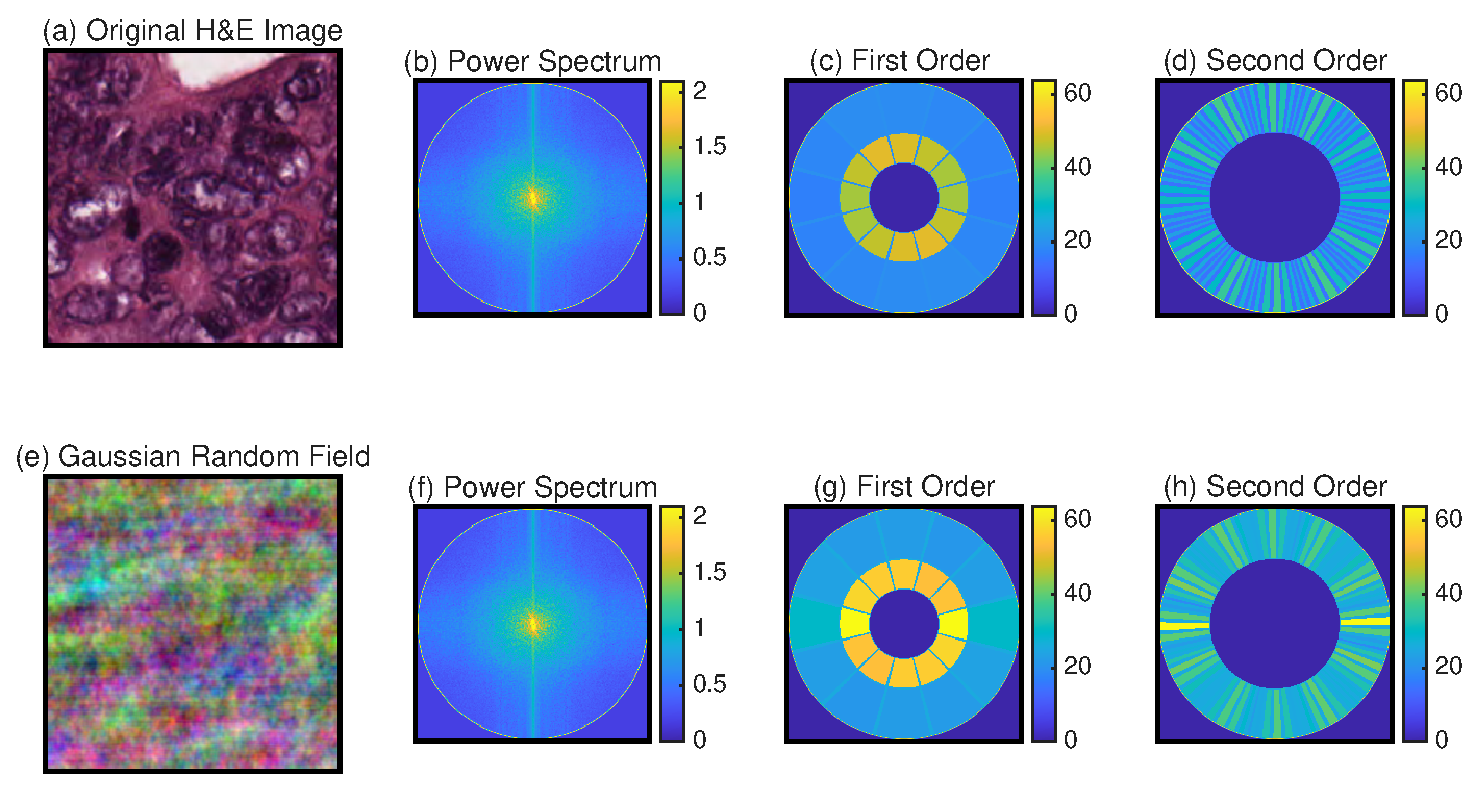
\includegraphics[width=\textwidth]{ScatteringDisks_Comparison.eps}
\caption{Scattering coefficients of a tumor tissue patch versus a realization of Gaussian random field. Top row: Original H\&E image of tumor (a), its power spectrum (b), first-order (c) and second-order (d) scattering coefficients. Bottom row: a realization of Gaussian random field with power spectrum (e-f) and its scattering coefficients (g-h). Identical power spectra (b, f) but different scattering coefficients.}
\label{fig:spectrum}
\end{figure}

%
\section{Methodology}

\subsection{Scattering Network Architecture}

A two-layer scattering network is created because the energy within scattering coefficients decays exponentially with layer depth~\cite{waldspurger2017exponential}, and third- and higher-order coefficients typically contain less than one percent of the input energy~\cite{bruna2013invariant}. An example architecture of a wavelet scattering tree is illustrated in Figure ~\ref{fig:network}. 

\begin{figure}[h!]
    \begin{center}
    \includegraphics[width=1.0\textwidth]{Images/scat_tree_dark_green.pdf}
    \caption{Two-layer scattering tree. Green nodes: scattering coefficients; white nodes: intermediate wavelet modulus coefficients.}
    \label{fig:network}
    \end{center}
\end{figure}




The scaling function $\phi$ has a spatial support of 20 pixels, providing translation invariance and serving as the lowpass filter for spatial averaging. The wavelet filter bank uses two dyadic scales in each layer, capturing features at fine and coarse resolutions, with six orientations uniformly sampled in $[0,\pi)$ at angles $\theta_\ell = \ell\pi/6$ for $\ell = 0,1,2,3,4,5$. Each filter bank thus contains $N_1 = N_2 = 12$ filters, organized as 2 scales $\times$ 6 orientations. These parameters were chosen heuristically through experimentation. Morlet spatial filters that are used in the first filter bank are shown in Figure~\ref{fig:morlet_fb}. 

\begin{figure}[htb!]
\centering

\includegraphics[width=\textwidth]{Images/wavelets_J2_angles6.pdf}
\caption{Morlet Spatial Filters in the first filter bank for each combination of $\lambda_1$ and $\theta_1$}
\label{fig:morlet_fb}
\end{figure}

With 12 filters in the first layer, we obtain 12 first-order scattering coefficients. The maximum number of second-order coefficients would be $12 \times 12 = 144$, giving a theoretical total of $1 + 12 + 144 = 157$ coefficients. However, the scattering feature vector contains only 49 coefficients due to a path retention constraint based on spectral overlap. When the magnitude spectra of $|f \ast \psi_{\lambda_1,\theta_1}(\mathbf{x})|$ and $\psi_{\lambda_2,\theta_2}$ do not overlap significantly in the frequency domain, the corresponding second-order coefficient $\big||f \ast \psi_{\lambda_1,\theta_1}(\mathbf{x})| \ast \psi_{\lambda_2,\theta_2}(\mathbf{x})\big| \ast \phi(\mathbf{x})$ is negligible and can be discarded~\cite{anden2014deep}. Specifically, second-order paths are retained only when $\lambda_1 < \lambda_2$, ensuring that the second wavelet operates at a coarser scale (lower frequency) than the first. This frequency-decreasing constraint is fundamental to the scattering transform architecture, as it ensures that each subsequent layer captures progressively coarser features. Among the 144 potential second-order paths, only those satisfying $\lambda_1 < \lambda_2$ are retained, reducing the count to 36 non-negligible second-order coefficients. This yields a final feature vector of dimension $1 + 12 + 36 = 49$. 

\subsection{Implementation}

The dataset was divided into a training set (4000 images) and testing set (1000 images), with each tissue type equally represented (500 training, 125 test images per type). Each image was transformed into a scattering feature vector of size $1 \times 49$, yielding training and test feature matrices of dimensions $4000 \times 49$ and $1000 \times 49$, respectively.

A Support Vector Machine (SVM) with cubic polynomial kernel was trained using one-versus-all multiclass classification. Columns of the training feature matrix were z-score standardized prior to training. The workflow is shown in Figure~\ref{fig:workflow}. The complete analysis was performed using MATLAB 2025b~\cite{matlab2023} with Wavelet Toolbox, Statistics and Machine Learning Toolbox, and Parallel Computing Toolbox. All computations were performed on a MacBook Pro with Apple M3 Pro chip containing 11 cores, 18 GB unified memory.

\begin{figure}[h!]
\centering
\includegraphics[width = 0.8\textwidth]{Images/Workflow_scat.pdf}
\caption{Classification workflow showing training and testing phases.}
\label{fig:workflow}
\end{figure}

%
\section{Results}

The classifier achieved 81.60\% mean accuracy via 10-fold cross-validation on the training set. On the held-out test set, the model demonstrated 85.10\% accuracy with balanced precision (85.19\%), recall (85.10\%), and F1-score (85.08\%). Computational efficiency was notable: feature extraction required 2.42 minutes for all test images, training completed in 23.82 seconds, and prediction took only 0.04 seconds. Table~\ref{tab:results} presents detailed per-class performance metrics.

The confusion matrix (Figure~\ref{fig:confusion}) reveals substantial variation in per-class classification accuracy achieved by the model. The model perfectly classified the empty background (100.0\%), while adipose tissue was classified with near-perfect accuracy (96.8\%), reflecting their distinctive and relatively homogeneous textural patterns. Tumor epithelium was classified with an accuracy of 88.8\%, which is a clinically favorable characteristic for cancer detection applications. The model achieved strong classification performance for lymphocytes (84.0\%), debris (82.4\%), and simple stroma (82.4\%). The most challenging tissue types for the model were complex stroma (70.4\%) and mucosa (76.0\%), likely due to their heterogeneous cellular compositions and structural similarities to other tissue types.

\begin{table}[h]
\centering
\caption{Per-class performance metrics on test set (125 samples per class).}
\label{tab:results}
\begin{tabular}{l@{\hspace{1cm}}c@{\hspace{1cm}}c@{\hspace{1cm}}c}
\toprule
\textbf{Tissue} & \textbf{Accuracy (Recall)} & \textbf{Precision} & \textbf{F1-Score} \\
\midrule
Tumor & 88.80\% & 82.22\% & 85.38\% \\
Stroma & 82.40\% & 89.91\% & 83.76\% \\
Complex & 70.40\% & 72.03\% & 69.96\% \\
Lympho & 84.00\% & 87.50\% & 85.71\% \\
Debris & 82.40\% & 79.55\% & 81.71\% \\
Mucosa & 76.00\% & 74.62\% & 76.08\% \\
Adipose & 96.80\% & 94.40\% & 94.40\% \\
Empty & 100.00\% & 93.89\% & 96.09\% \\
\midrule
Average & 85.10\% & 84.26\% & 84.14\% \\
\bottomrule
\end{tabular}
\end{table}

\begin{figure}[h]
\centering
\includegraphics[width = \textwidth]{Images/Confusion_matrix.pdf}
\caption{Confusion matrix illustrating the classification results on the test dataset.}
\label{fig:confusion}
\end{figure}

%
\section{Discussion}

To our knowledge, this work represents the first application of wavelet scattering transforms to histopathology tissue classification. Our results demonstrate that scattering features extracted through a mathematically principled, training-free process achieve competitive performance on this challenging eight-class colorectal cancer tissue classification task. The 85.10\% test accuracy is particularly noteworthy given that the method requires no iterative optimization or large annotated training datasets, addressing a critical bottleneck in medical image analysis where labeled data is often scarce and expensive to obtain.

The structural similarities between scattering networks and convolutional neural networks provide theoretical insight into why wavelet-based features perform well for tissue classification. As illustrated in Figure~\ref{fig:comparison}, both architectures share three fundamental operations: convolution (using wavelets in scattering vs. learned kernels in CNNs), a  nonlinearity operation (modulus in scattering vs. ReLU in CNNs), and averaging with a scaling function (analogous to pooling in CNNs)~\cite{mallat2016understanding}. 

\begin{figure}[h!]
\centering
\includegraphics[width = \textwidth]{Images/cnn_scatter_comp.pdf}
\caption{Similarities between operations in convolutional network and wavelet scattering network. Both architectures cascade these three operations across multiple layers}
\label{fig:comparison}
\end{figure}

However, scattering networks employ predefined Morlet wavelets rather than learned filters, eliminating the need for  training in the feature extraction process while providing mathematical guarantees of translation invariance and Lipschitz continuity to deformations~\cite{mallat2012group,bruna2013invariant}.  For our colorectal tissue classification task, second-order scattering coefficients ($m=2$) capture scale interactions and 4th-order moments that effectively discriminate the complex textural patterns characteristic of different tissue types. As previously noted, this approach is computationally very efficient as extracting features for the entire training and test set took just 2.42 minutes, while training the multi-class SVM was completed in only 23.82 seconds.

A few limitations should be acknowledged. The wavelets are predefined rather than learned from data, potentially limiting adaptability to dataset-specific characteristics. Our future objective is to tackle this limitation by developing wavelets learned directly from image data to effectively capture the structures present in the histology tissue types and improve the classification accuracy. Validation on additional multi-center datasets is needed to assess generalization beyond the single dataset used here. Finally, the patch-based analysis does not consider whole-slide spatial context or relationships between neighboring tissue regions.


%
\section{Acknowledgments}

No funding was received for conducting this study. The authors have no relevant financial or non-financial interests to disclose. The research was supported by an intramural NIH grant 889286 Clinical Center's Research Award for Staff Clinicians (E.L.).




\subsection*{Availability of Code and Materials}
All code and materials supporting this work are publicly available on GitHub to facilitate reproducibility:

\vspace{0.1cm}
\noindent
\faGithub~\textbf{Analysis Code:} \href{https://github.com/rrmaram2000/AIPR_Codes}{\texttt{rrmaram2000/AIPR\_Codes}}\\
\textit{MATLAB codes for reproducing results and figures}

\vspace{0.1cm}
\noindent
\faGithub~\textbf{Manuscript Source:} \href{https://github.com/rrmaram2000/AIPR_2025_Writing}{\texttt{rrmaram2000/AIPR\_2025\_Writing}}\\
\textit{LaTeX source files, figures, and supplementary materials}

%
\bibliographystyle{splncs04}
\begin{thebibliography}{20}

\bibitem{mezheyeuski2016image}
Mezheyeuski, A., Hrynchyk, I., Karlberg, M., et al.: Image analysis-derived metrics of histomorphological complexity predicts prognosis and treatment response in stage II-III colon cancer. Sci. Rep. \textbf{6}, 36149 (2016)

\bibitem{zhou2019immune}
Zhou, R., Zhang, J., Zeng, D., et al.: Immune cell infiltration as a biomarker for the diagnosis and prognosis of stage I-III colon cancer. Cancer Immunol. Immunother. \textbf{68}, 433--442 (2019)

\bibitem{lubner2015ct}
Lubner, M.G., Stabo, N., Lubner, S.J., et al.: CT textural analysis of hepatic metastatic colorectal cancer: pre-treatment tumor heterogeneity correlates with pathology and clinical outcomes. Abdom. Imaging \textbf{40}, 2331--2337 (2015)

\bibitem{jin2022combinatory}
Jin, H.-Y., Yoo, S.-Y., Lee, J.-A., et al.: Combinatory statuses of tumor stromal percentage and tumor infiltrating lymphocytes as prognostic factors in stage III colorectal cancers. J. Gastroenterol. Hepatol. \textbf{37}, 551--557 (2022)

\bibitem{alic2014quantification}
Alic, L., Niessen, W.J., Veenland, J.F.: Quantification of Heterogeneity as a Biomarker in Tumor Imaging: A Systematic Review. PLoS ONE \textbf{9}, e110300 (2014)

\bibitem{kather2016multi}
Kather, J.N., Weis, C.-A., Bianconi, F., et al.: Multi-class texture analysis in colorectal cancer histology. Sci. Rep. \textbf{6}, 27988 (2016)

\bibitem{mallat2008wavelet}
Mallat, S.: A Wavelet Tour of Signal Processing, Third Edition: The Sparse Way. Academic Press (2008)

\bibitem{anden2019joint}
Andén, J., Lostanlen, V., Mallat, S.: Joint Time–Frequency Scattering. IEEE Trans. Signal Process. \textbf{67}, 3704--3718 (2019)

\bibitem{mallat2012group}
Mallat, S.: Group Invariant Scattering. Commun. Pure Appl. Math. \textbf{65}(10), 1331--1398 (2012)

\bibitem{mallat2016understanding}
Mallat, S.: Understanding deep convolutional networks. Phil. Trans. R. Soc. A \textbf{374}, 20150203 (2016)

\bibitem{anden2011multiscale}
Andén, J., Mallat, S.: Multiscale scattering for audio classification. In: 12th Int. Society for Music Information Retrieval Conf., ISMIR 2011, pp. 657--662 (2011)

\bibitem{bruna2011classification}
Bruna, J., Mallat, S.: Classification with scattering operators. In: CVPR 2011, pp. 1561--1566 (2011)

\bibitem{baharlouei2023wavelet}
Baharlouei, Z., Rabbani, H., Plonka, G.: Wavelet scattering transform application in classification of retinal abnormalities using OCT images. Sci. Rep. \textbf{13}, 19013 (2023)

\bibitem{agboola2023wavelet}
Agboola, H.A., Zaccheus, J.E.: Wavelet image scattering based glaucoma detection. BMC Biomed. Eng. \textbf{5}(1), 1 (2023)

\bibitem{waldspurger2017exponential}
Waldspurger, I.: Exponential decay of scattering coefficients. In: 2017 Int. Conf. on Sampling Theory and Applications (SampTA), pp. 143--146 (2017)

\bibitem{bruna2013invariant}
Bruna, J., Mallat, S.: Invariant Scattering Convolution Networks. IEEE Trans. Pattern Anal. Mach. Intell. \textbf{35}, 1872--1886 (2013)

\bibitem{anden2014deep}
Andén, J., Mallat, S.: Deep Scattering Spectrum. IEEE Trans. Signal Process. \textbf{62}, 4114--4128 (2014)

\bibitem{matlab2023}
MATLAB version: 25.2 (R2025b). The MathWorks Inc., Natick, Massachusetts (2025)

\end{thebibliography}

\end{document}